% ****** Start of file apssamp.tex ******
%
%   This file is part of the APS files in the REVTeX 4.2 distribution.
%   Version 4.2a of REVTeX, December 2014
%
%   Copyright (c) 2014 The American Physical Society.
%
%   See the REVTeX 4 README file for restrictions and more information.
%
% TeX'ing this file requires that you have AMS-LaTeX 2.0 installed
% as well as the rest of the prerequisites for REVTeX 4.2
%
% See the REVTeX 4 README file
% It also requires running BibTeX. The commands are as follows:
%
%  1)  latex apssamp.tex
%  2)  bibtex apssamp
%  3)  latex apssamp.tex
%  4)  latex apssamp.tex
%
\documentclass[%
 reprint,
%superscriptaddress,
%groupedaddress,
%unsortedaddress,
%runinaddress,
%frontmatterverbose, 
%preprint,
%preprintnumbers,
%nofootinbib,
%nobibnotes,
%bibnotes,
 amsmath,amssymb,
 aps,
%pra,
%prb,
%rmp,
%prstab,
%prstper,
%floatfix,
]{revtex4-2}

\usepackage{graphicx}% Include figure files
\usepackage{dcolumn}% Align table columns on decimal point
\usepackage{bm}% bold math
\usepackage{hyperref}% add hypertext capabilities
\usepackage{caption}
\usepackage{subcaption}
%\usepackage[mathlines]{lineno}% Enable numbering of text and display math
%\linenumbers\relax % Commence numbering lines

%\usepackage[showframe,%Uncomment any one of the following lines to test 
%%scale=0.7, marginratio={1:1, 2:3}, ignoreall,% default settings
%%text={7in,10in},centering,
%%margin=1.5in,
%%total={6.5in,8.75in}, top=1.2in, left=0.9in, includefoot,
%%height=10in,a5paper,hmargin={3cm,0.8in},
%]{geometry}

\begin{document}

\preprint{APS/123-QED}

\title{Elementary Particle Physics (PHY451): \\ "short" exercise}

\author{Yuri van der Burg}
 \email{yuri.vanderburg@uzh.ch}
\affiliation{University of Zurich}

\date{\today}

\begin{abstract}
In this short exercise, a dataset from the CMS experiment, as well as a Monte Carlo (MC) simulation of various processes, are provided. They together are used to search for the semi-leptonic decay of the top quark, $t \bar t \rightarrow \mu \nu b \bar b q \bar q$. An optimal cut was selected and the cross-section of this decay was calculated. The charge asymmetry of the W-boson was determined for different ranges of pseudorapidity. Both cross-section and W-boson charge asymmetry agree with the literature. 
\end{abstract}
\maketitle

%\tableofcontents

\section{\label{sec:introduction}Introduction}
With its mass of 173 GeV/c$^2$, the top quark is the heaviest elementary particle. Its long lifetime of about $5 \cdot 10^{-25}$s makes it possible to study the top quark in great detail \cite{workman_review_2022}.
The semi-leptonic decay of $t \bar t$ consists of the decay mode $t \rightarrow bW$, where one of the $W$ bosons decays leptonically $W \rightarrow \mu \nu$ and the other decays hadronically $W \rightarrow q \bar q$ \cite{cms_collaboration_measurement_2018}. The total decay is $t \bar t \rightarrow \mu \nu b \bar b q \bar q$. \\
The cross-section of this decay can be calculated as in equation (\ref{eq:cross_sec}):

\begin{equation}\label{eq:cross_sec}
    \sigma = \frac{N}{L \cdot \epsilon \cdot A}
\end{equation}

Here, $N$ is the total number of events, $L$ the luminosity, $\epsilon$ the trigger efficiency, and $A$ the acceptance. \\
In this process we expect a charge asymmetry of the W-boson, because the Large Hadron Collider at CERN is a pp-collider. The W-boson charge asymmetry is very difficult to measure, therefore we measure the lepton charge asymmetry ($W \rightarrow \mu \nu$) and identify the lepton charge with the W charge asymmetry $\mathcal{A}$. It is given by equation \ref{eq:charge_asym}, where $N_{\pm}$ indicates the number of events with a $\mu^{\pm}$. 


\begin{equation}\label{eq:charge_asym}
    \mathcal{A} = \frac{N_+ - N_-}{N_+ + N_-}
\end{equation}


\section{\label{sec:}Event simulation and selection}
The data samples were provided by Dr. Stefanos Leontsinis and originate from a CMS experiment with 50 pb$^{-1}$ data collected at an energy of 7 TeV. The event simulation (Monte Carlo) was provided as well. 
The analysis was done in \textsc{PYTHON}, using the \textsc{ROOT} framework. The codes can be found on GitHub. \footnote{\url{https://github.com/Yurivanderburg/EPP_Project}} 


\subsection{\label{sec:}Event selection}
The event selection was conducted by optimizing the score, defined as in equation (\ref{eq:score}), on the Monte Carlo simulated data. This provides a quantitative estimation of how much background is present in the signal. The uncertainty is given in equation (\ref{eq:score_err}).

\begin{equation}\label{eq:score}
    \varsigma = \frac{S}{\sqrt{S + B}}
\end{equation}


\subsection{Cut selection}
In a first step different cuts were selected. This was done qualitatively by looking at different parameter distributions. The cuts used including its numerical value can be found in table \ref{tab:optimal_params}. With exception of the number of isolated muon, they are lower limits. \\
These parameters are justified physically because in the desired events we do expect an isolated muon with its corresponding neutrino, which appears as missing transverse energy (MET). The other W-boson decays into an $q \bar q$ pair, corresponding to two jets, as they have relatively high energy. There should also be at least one b-jet present.  

\begin{table}[b]
    \centering
    \begin{tabular}{|c|c|}
    \hline
    Parameter            & Cut value \\
    \hline
    B-tagged jets        &  1 \\
    Total jets           &  4 \\
    Missing energy       &  30 GeV \\
    Muon tranv. momentum &  20 GeV \\
    Isolated muons       &  1 \\
    \hline
    \end{tabular}
    \caption{Parameters that yield the highest score $\varsigma$. }
    \label{tab:optimal_params}
\end{table}


\subsection{Cut optimization}
In a second step, the selected cuts were systematically scanned over a wide range to find the highest score $\varrho$, which was obtained with the parameters indicated in table \ref{tab:optimal_params}. 
Figure \ref{fig:cut_param} show the effect of the different parameters on the score. We can see that the score decreases significantly when the cuts are very strict because we cut off a large portion of the signal as well. 
Figure \ref{fig:muon_pt} shows the transverse momentum of the muons. The main background comes from single-top events. 

\begin{figure}
    \centering
    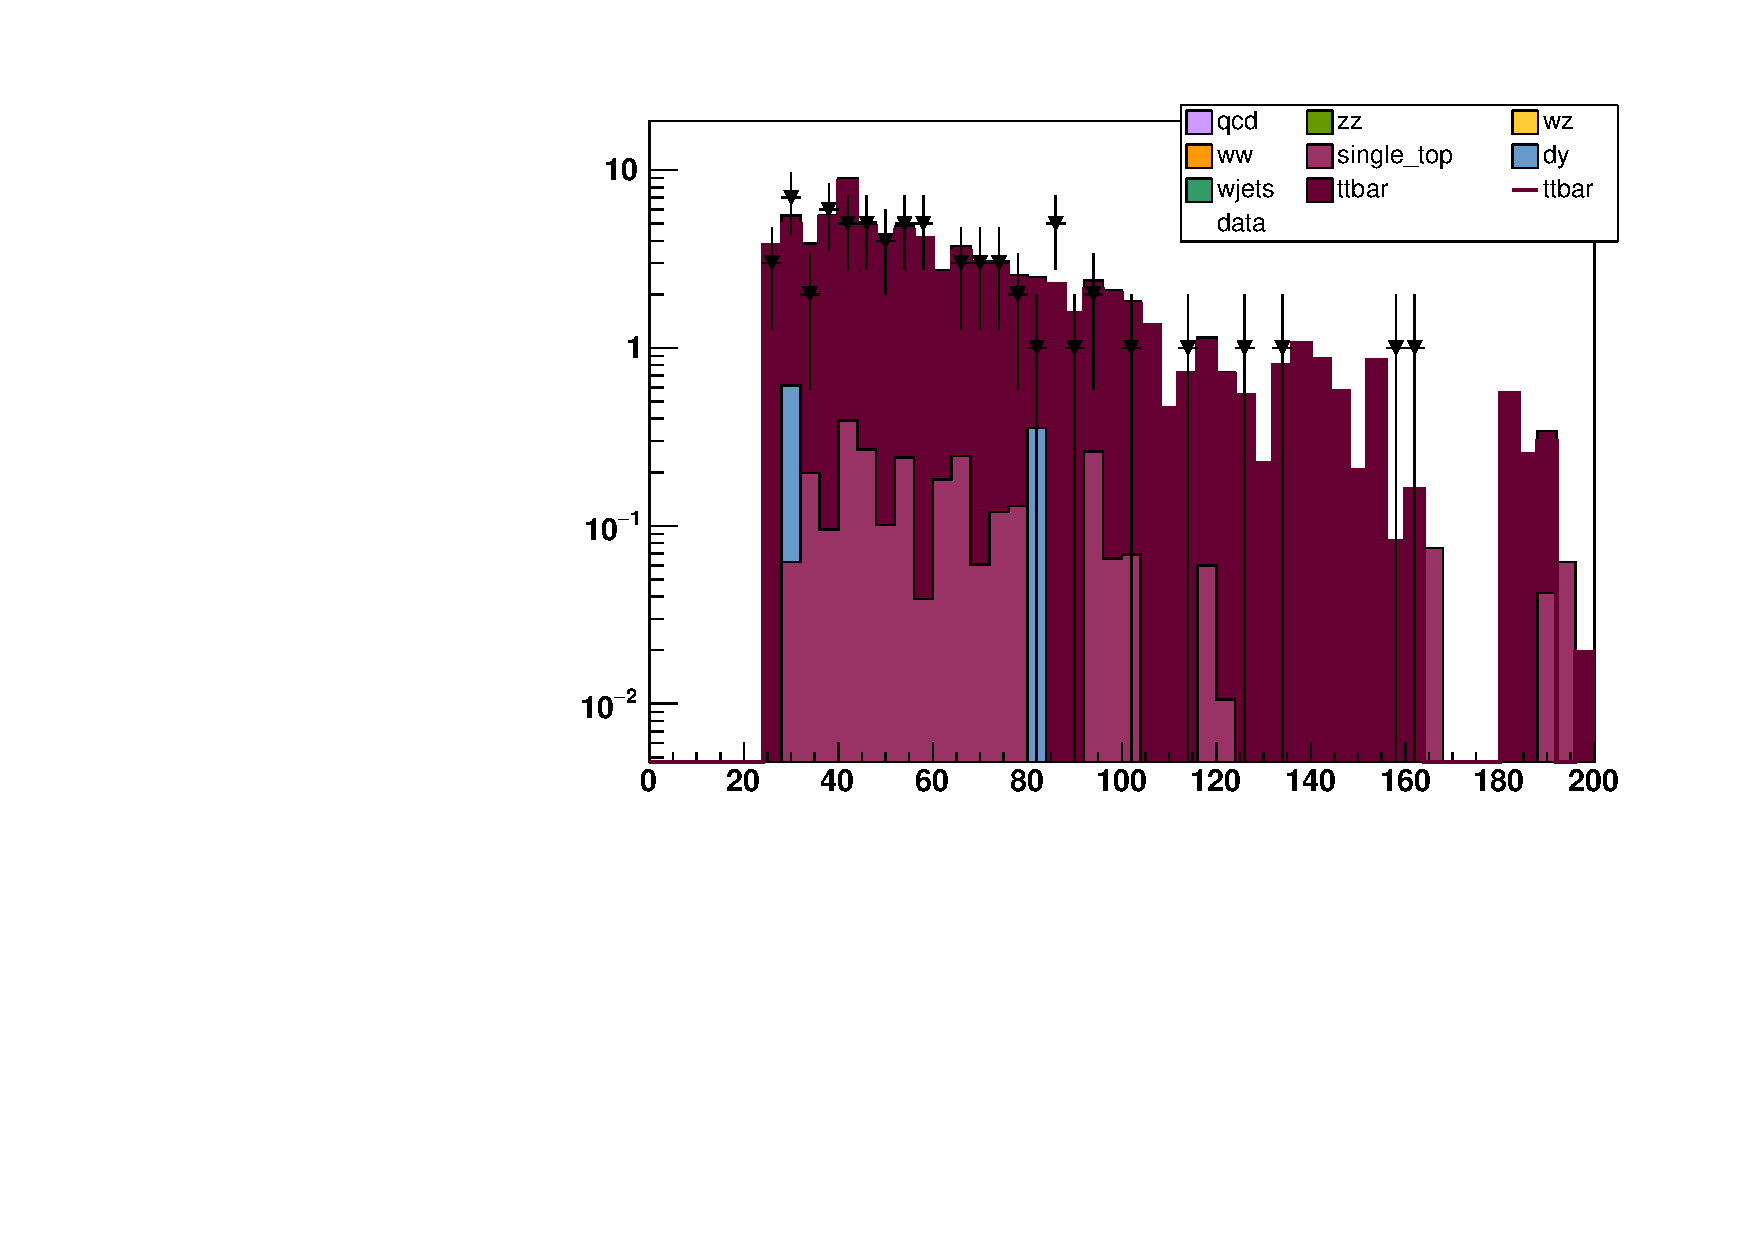
\includegraphics[width=0.5\textwidth]{Plots/part1/Muon_Pt.pdf}
    \caption{Transverse momentum of the muons identified in the $t \bar t \rightarrow \mu \nu b \bar b q \bar q$ process. The dominant background comes from single-top events.}
    \label{fig:muon_pt}
\end{figure}

\section{Cross section calculation}
The selected cuts are then applied to the dataset. From the MC simulation, we do expect $(18 \pm 4)$ background events. When this is subtracted from the dataset, we do get a total of $(146.6 \pm 8.5)$ observed events. This corresponds to a detector acceptance (172 events) of $(2.2 \pm 0.1)$~\%. Furthermore, we assume a detector efficiency of $(87 \pm 5)\%$ and a systematic uncertainty of 10\%. 
The total cross-section for this event is $(155.6~\pm~21.0$~(stat.)~$\pm~15.6$~(sys.)$)$~pb, achieving the theoretical cross-section of $(173.6 \pm 11.7)$~pb. This includes a 10\% uncertainty on the luminosity and the MC statistical uncertainty on the background, which follows the Poisson error $\sqrt{N}$. The cross-section is calculated using equation (\ref{eq:cross_sec}), the error using equation (\ref{eq:cross_sec_err}).


    
\section{W charge asymmetry}

For the calculation of the W charge asymmetry, only events containing muons with $p_T > 30$ GeV and neutrinos with MET $> 20$ GeV were selected. Since $\mathcal{A}$ depends on the pseudorapidity~$\eta$, it was determined in different regimes. 
In total, 3 fits were conducted to estimate the number of events containing a muon or an anti-muon:
The background was fitted using the error function, indicated in equations (\ref{eq:bkg_fit}) and (\ref{eq:erf}), on the MC simulated background. An example can be found in figure \ref{fig:fit_bkg}. It remains unclear why there seems to be some kind of signal at 60 GeV.  
The signal was fitted with a double Gaussian, shown in equations (\ref{eq:fit}) and (\ref{eq:gaus}). 

\begin{figure}
    \centering
    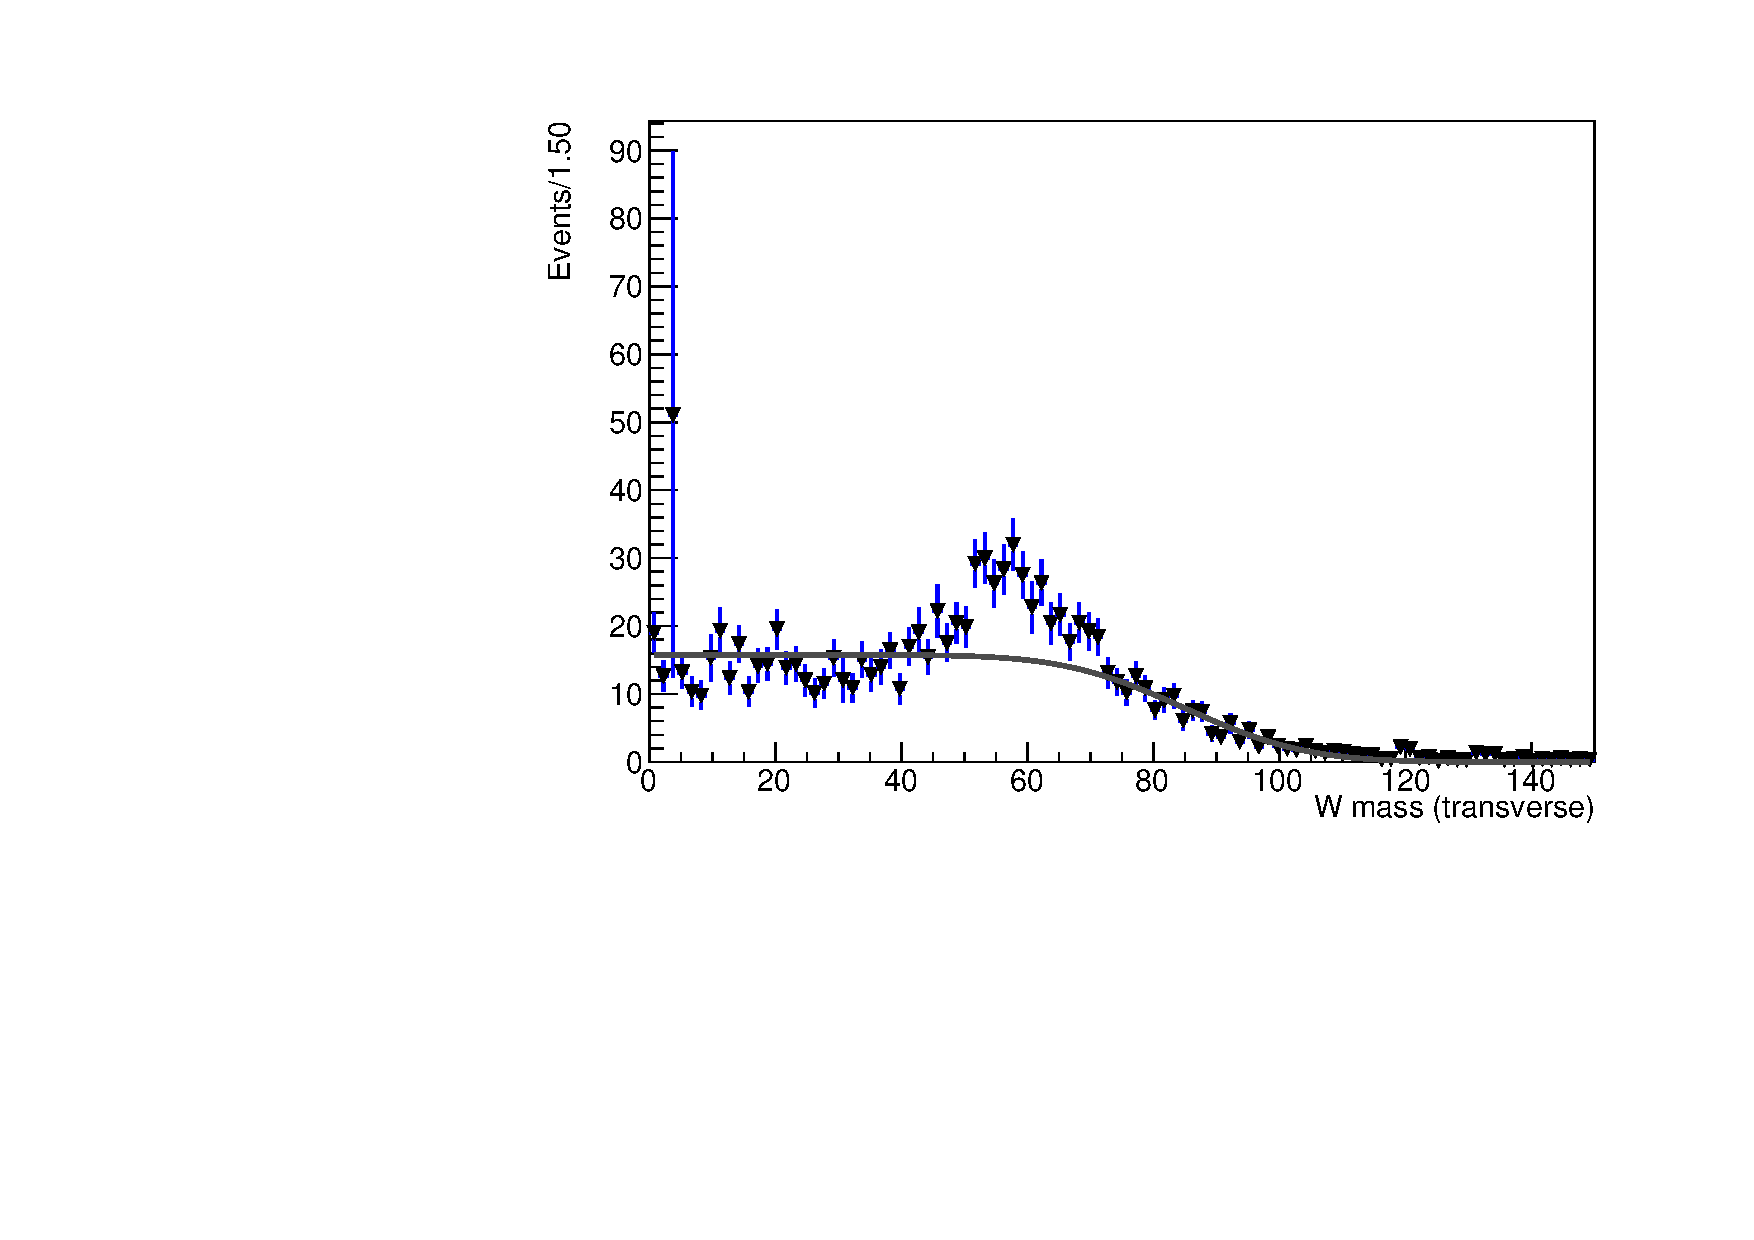
\includegraphics[width=0.45\textwidth]{Plots/part2/Background_fitpositive_0.pdf}
    \caption{Fit of an error function on the MC background surviving the selection. It corresponds to the selection of $\mu^+$ in the range $0 < \eta < 0.4$, hence this is the background fit used to model the background in figure \ref{fig:W_asym}, left row.}
    \label{fig:fit_bkg}
\end{figure}

\begin{equation}\label{eq:bkg_fit}
    b(x) = a \cdot \left( E \left(\frac{x - b}{c} \right) + 1 \right) 
\end{equation}

Here, $a$, $b$ and $c$ are fit parameters estimated with ROOT. The built-in error function is given by: 

\begin{equation}\label{eq:erf}
    E(x) = \frac{2}{\sqrt{\pi}} \int_0^x e^{-t^2} \, dt
\end{equation}

\begin{equation}\label{eq:fit}
    f(x) = \alpha \cdot G(x, \mu_1, \sigma_1) +  \beta \cdot G(x, \mu_2, \sigma_2)
\end{equation}

Again, $\alpha$ and $\beta$, as well as both $\mu_i$ and $\sigma_i$ are fit parameters. The Gaussians are given by:

\begin{equation}\label{eq:gaus}
    G(x) = \frac{1}{\sigma \sqrt{2 \pi}} e^{-\frac{1}{2} \left( \frac{x - \mu}{\sigma} \right)^2}
\end{equation}

\begin{figure}
    \centering
    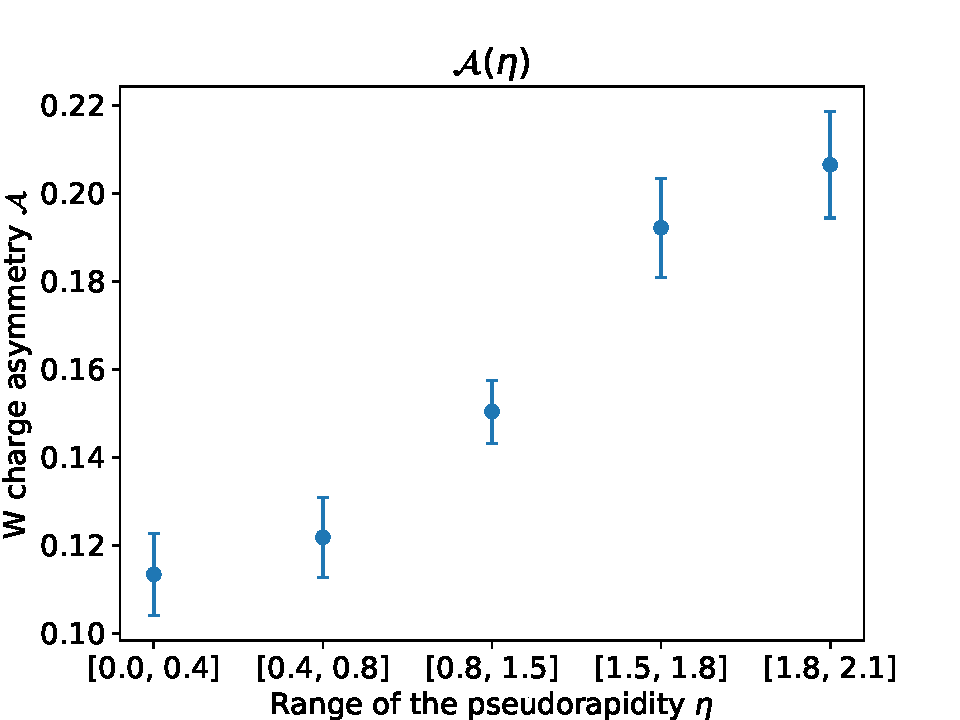
\includegraphics[width=0.5\textwidth]{Plots/part2/A_eta.pdf}
    \caption{W charge asymmetry for different ranges of the pseudorapidity $\eta$. There is clearly a trend that larger pseudorapidities lead to higher charge asymmetries.}
    \label{fig:A_eta}
\end{figure}



The final fit, consisting of the sum of two Gaussians and an error function, was done on the CMS data with the parameters obtained from the previous fits: Parameters $b$ and $c$ from the background fit were fixed, while the amplitude $a$ on the background, and all parameters of the Gaussians were used as starting parameters. The number of events was then estimated with the final fit function, evaluated as the value double Gaussian at the W-boson mass (80.4 GeV). 
The asymmetry and its unceratinty were then calculated using equations (\ref{eq:charge_asym}) and (\ref{eq:charge_asym_err}). The result for $\eta < 0.4$ is then $(11.3 \pm 0.9)$ \%. Table \ref{tab:asymmetry_etas} displays the different calculations for the charge asymmetry for different ranges of $\eta$, figure \ref{fig:A_eta} shows this graphically. 
The determined W charge asymmetries are very similar to the literature \cite{cms_collaboration_measurements_2020, saha_measurement_2013}.

\begin{table}
    \centering
    \begin{tabular}{|c|c|}
    \hline
    Range of $\eta$     & W Charge asymmetry [\%] \\
    \hline
    $[0.0, 0.4]$          & $(11.3 \pm 0.9)$ \\
    $[0.4, 0.8]$          & $(12.2 \pm 0.9)$ \\
    $[0.8, 1.5]$          & $(15.0 \pm 0.7)$ \\
    $[1.5, 1.8]$          & $(19.2 \pm 1.1)$ \\
    $[1.8, 2.1]$          & $(20.6 \pm 1.2)$ \\
    \hline
    \end{tabular}
    \caption{Ranges of $\eta$ and the corresponding W charge asymmetry.  }
    \label{tab:asymmetry_etas}
\end{table}




\begin{figure*}
        \centering
        \begin{subfigure}[b]{0.475\textwidth}
            \centering
            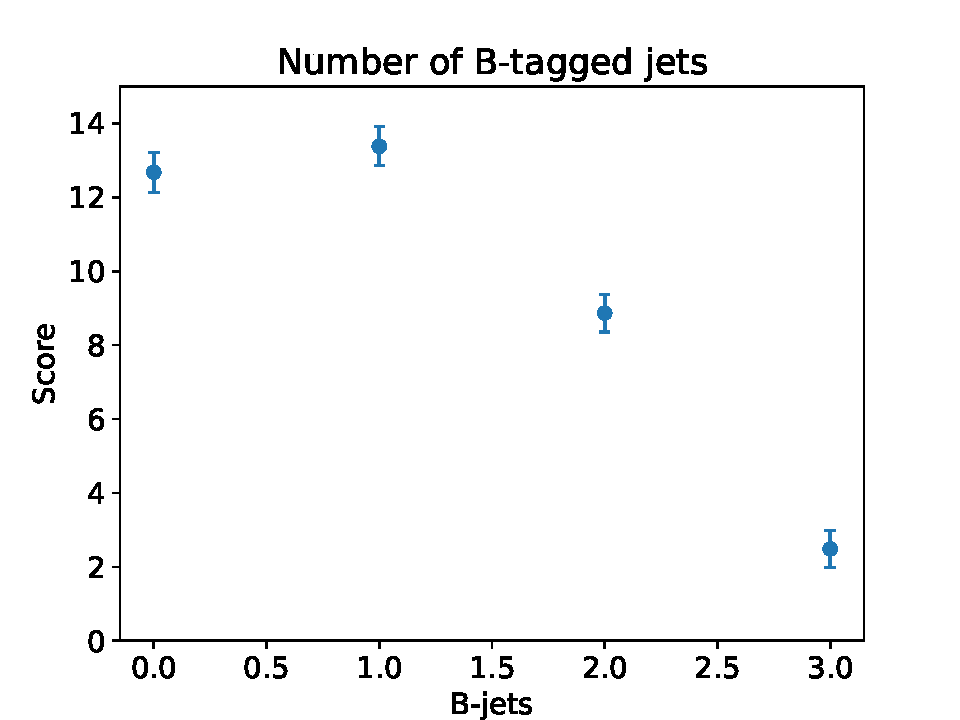
\includegraphics[width=\textwidth]{Plots/part1/Plot_Bjets.pdf}
            %\caption{Network 1}    
            \label{fig:mean and std of net14}
        \end{subfigure}
        \hfill
        \begin{subfigure}[b]{0.475\textwidth}  
            \centering 
            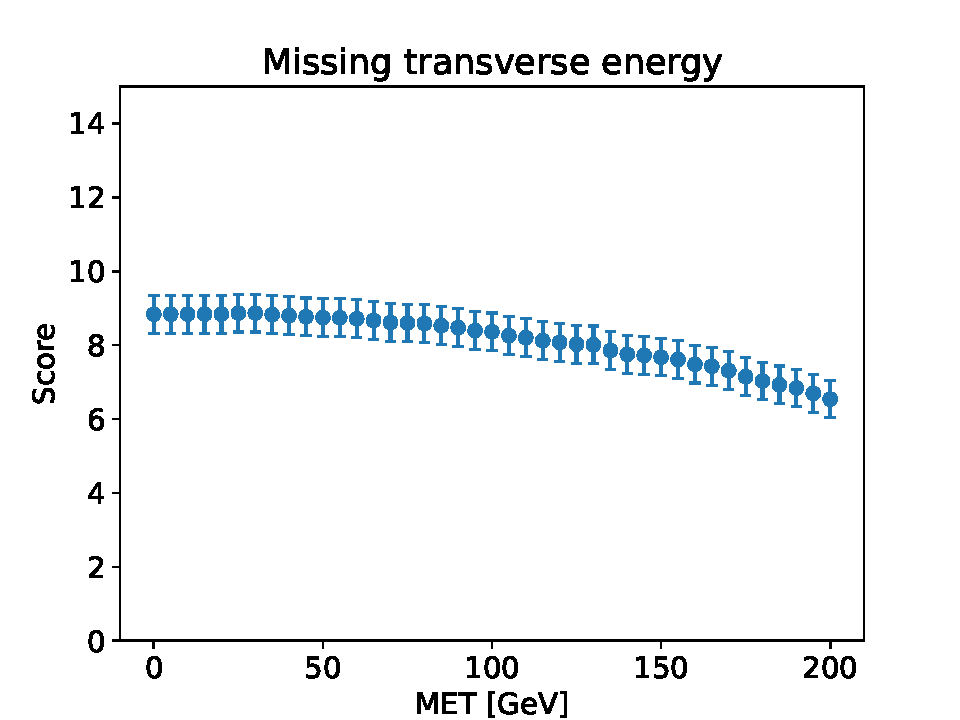
\includegraphics[width=\textwidth]{Plots/part1/Plot_MET.pdf}
            %\caption{Network 2} 
            \label{fig:mean and std of net24}
        \end{subfigure}
        \vskip\baselineskip
        \begin{subfigure}[b]{0.475\textwidth}   
            \centering 
            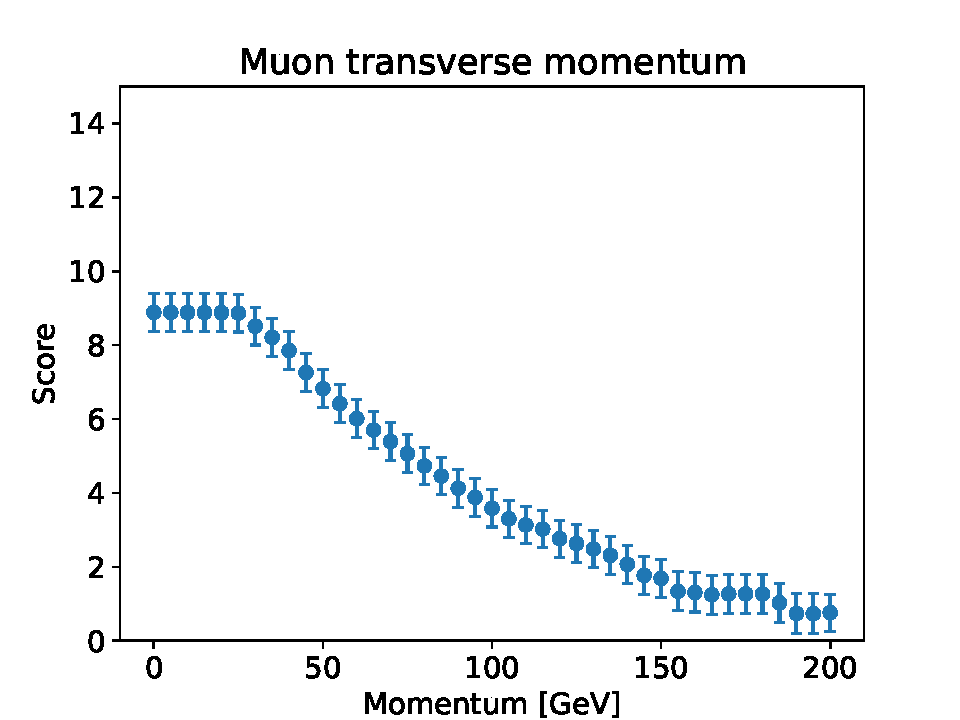
\includegraphics[width=\textwidth]{Plots/part1/Plot_MuonPT.pdf}
            %\caption{Netrwork n3}   
            \label{fig:mean and std of net34}
        \end{subfigure}
        \hfill
        \begin{subfigure}[b]{0.475\textwidth}   
            \centering 
            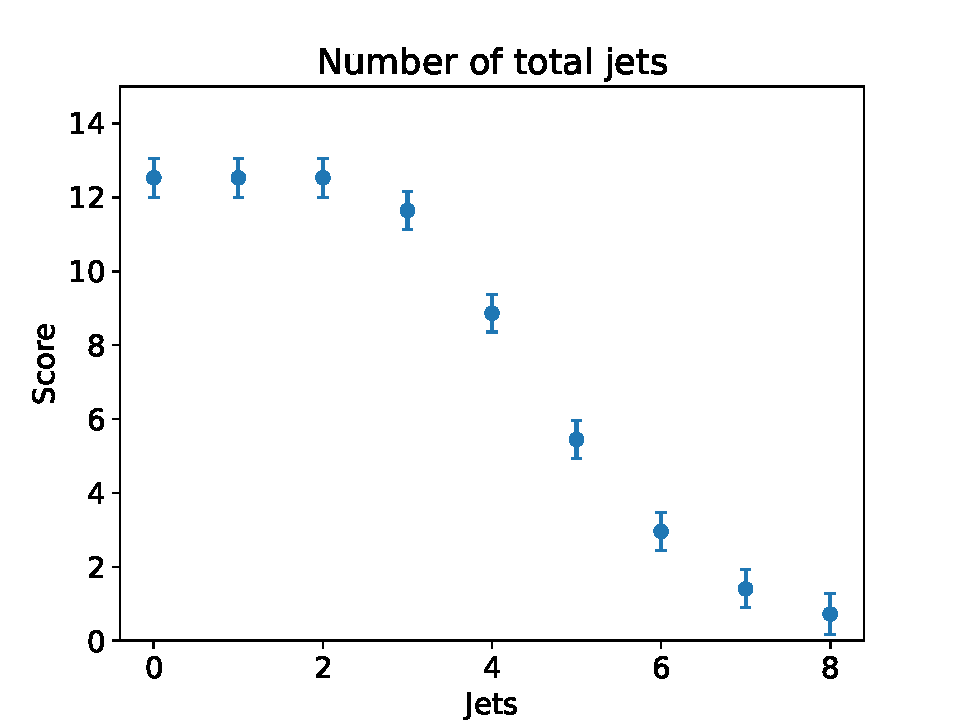
\includegraphics[width=\textwidth]{Plots/part1/Plot_Njets.pdf}
            %\caption{Network 4}   
            \label{fig:mean and std of net44}
        \end{subfigure}
        \caption{Plots indicating how the score $\varsigma$ depends on the different parameters. For each of the four cuts, all other three parameters were fixed according to table \ref{tab:optimal_params}. Generally, the score decreases if the cuts become too strict because neither signal nor background remains. If the score is not strict enough, the score increases, because though more background is included, even more signal is present.}
        \label{fig:cut_param}
    \end{figure*}


\begin{figure*}
        \centering
        \begin{subfigure}[b]{0.475\textwidth}
            \centering
            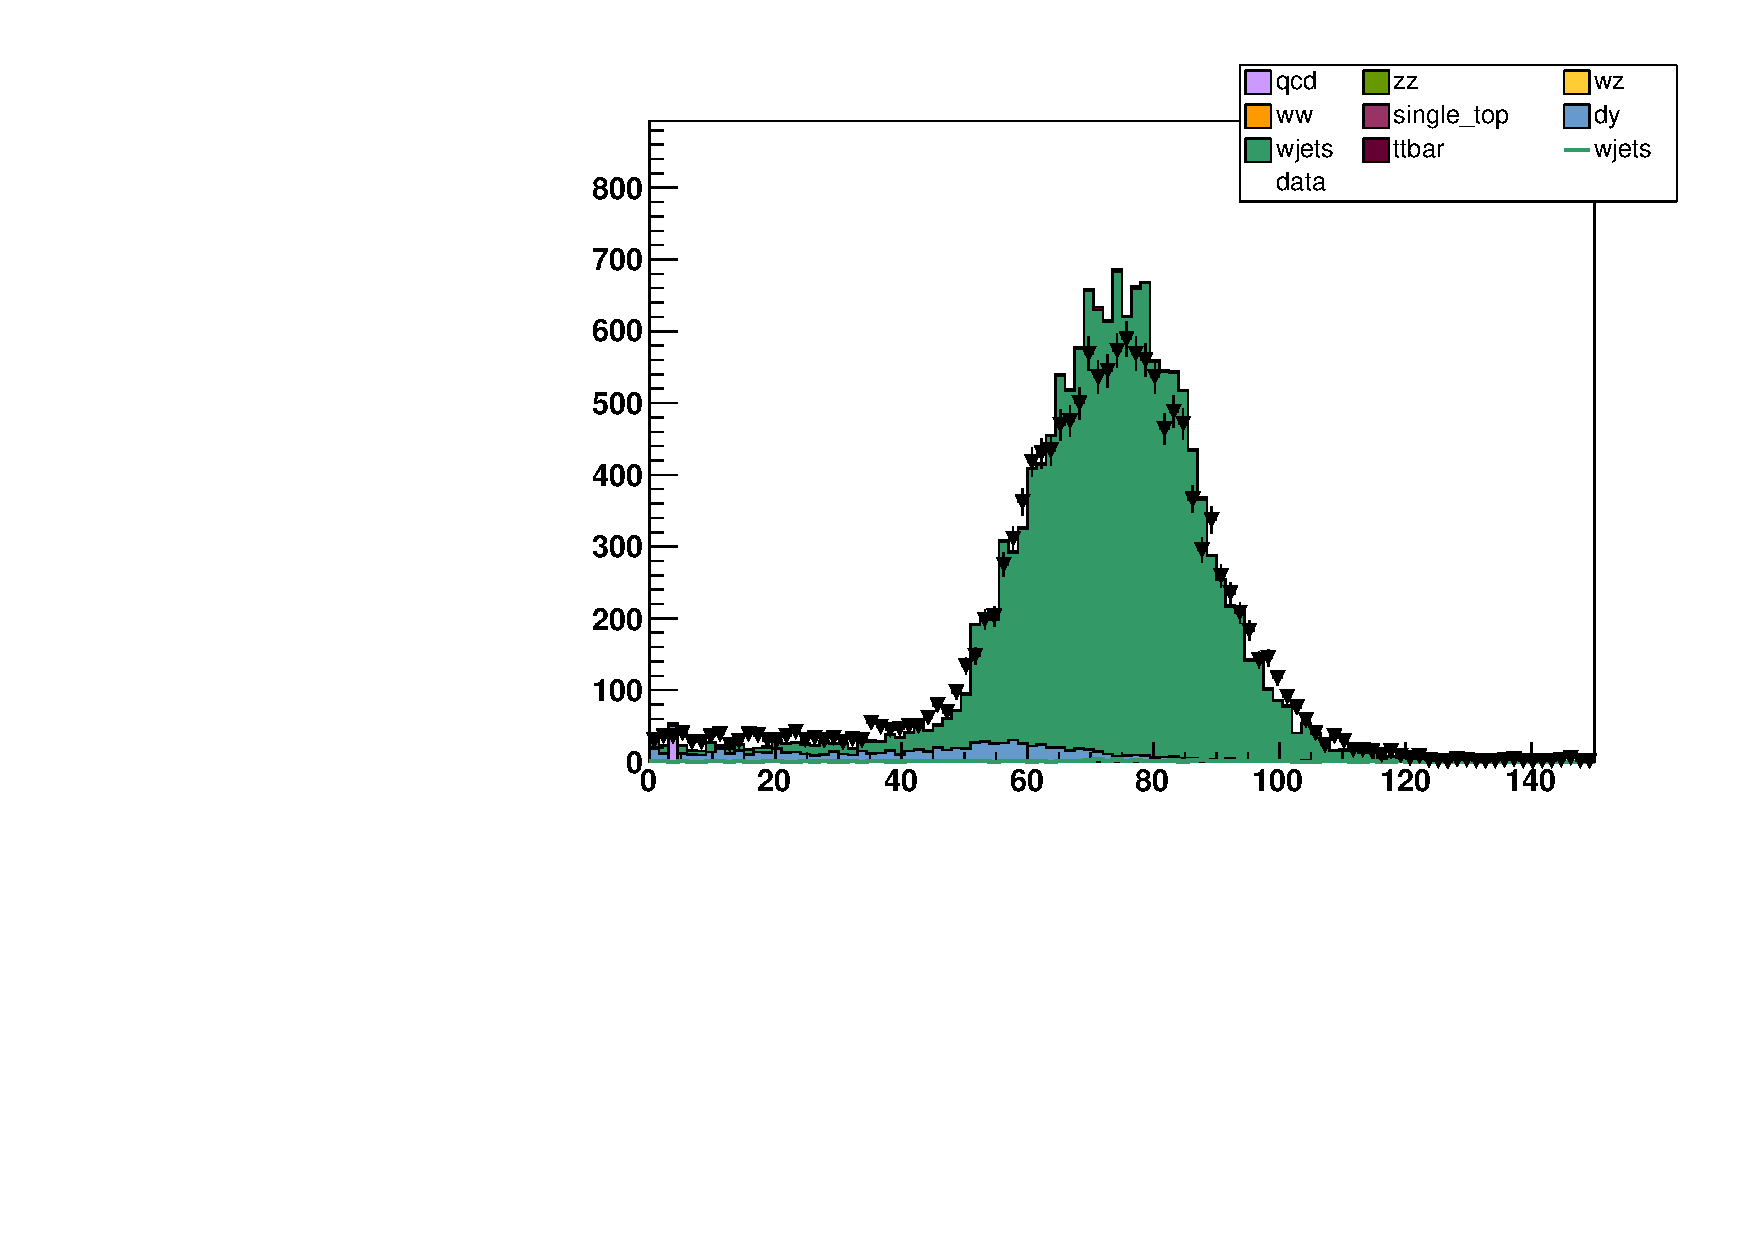
\includegraphics[width=\textwidth]{Plots/part2/W_mass_p.pdf}
            \caption{$W^+$-boson mass [GeV] distribution of the selected events.}    
            \label{fig:mean and std of net14}
        \end{subfigure}
        \hfill
        \begin{subfigure}[b]{0.475\textwidth}  
            \centering 
            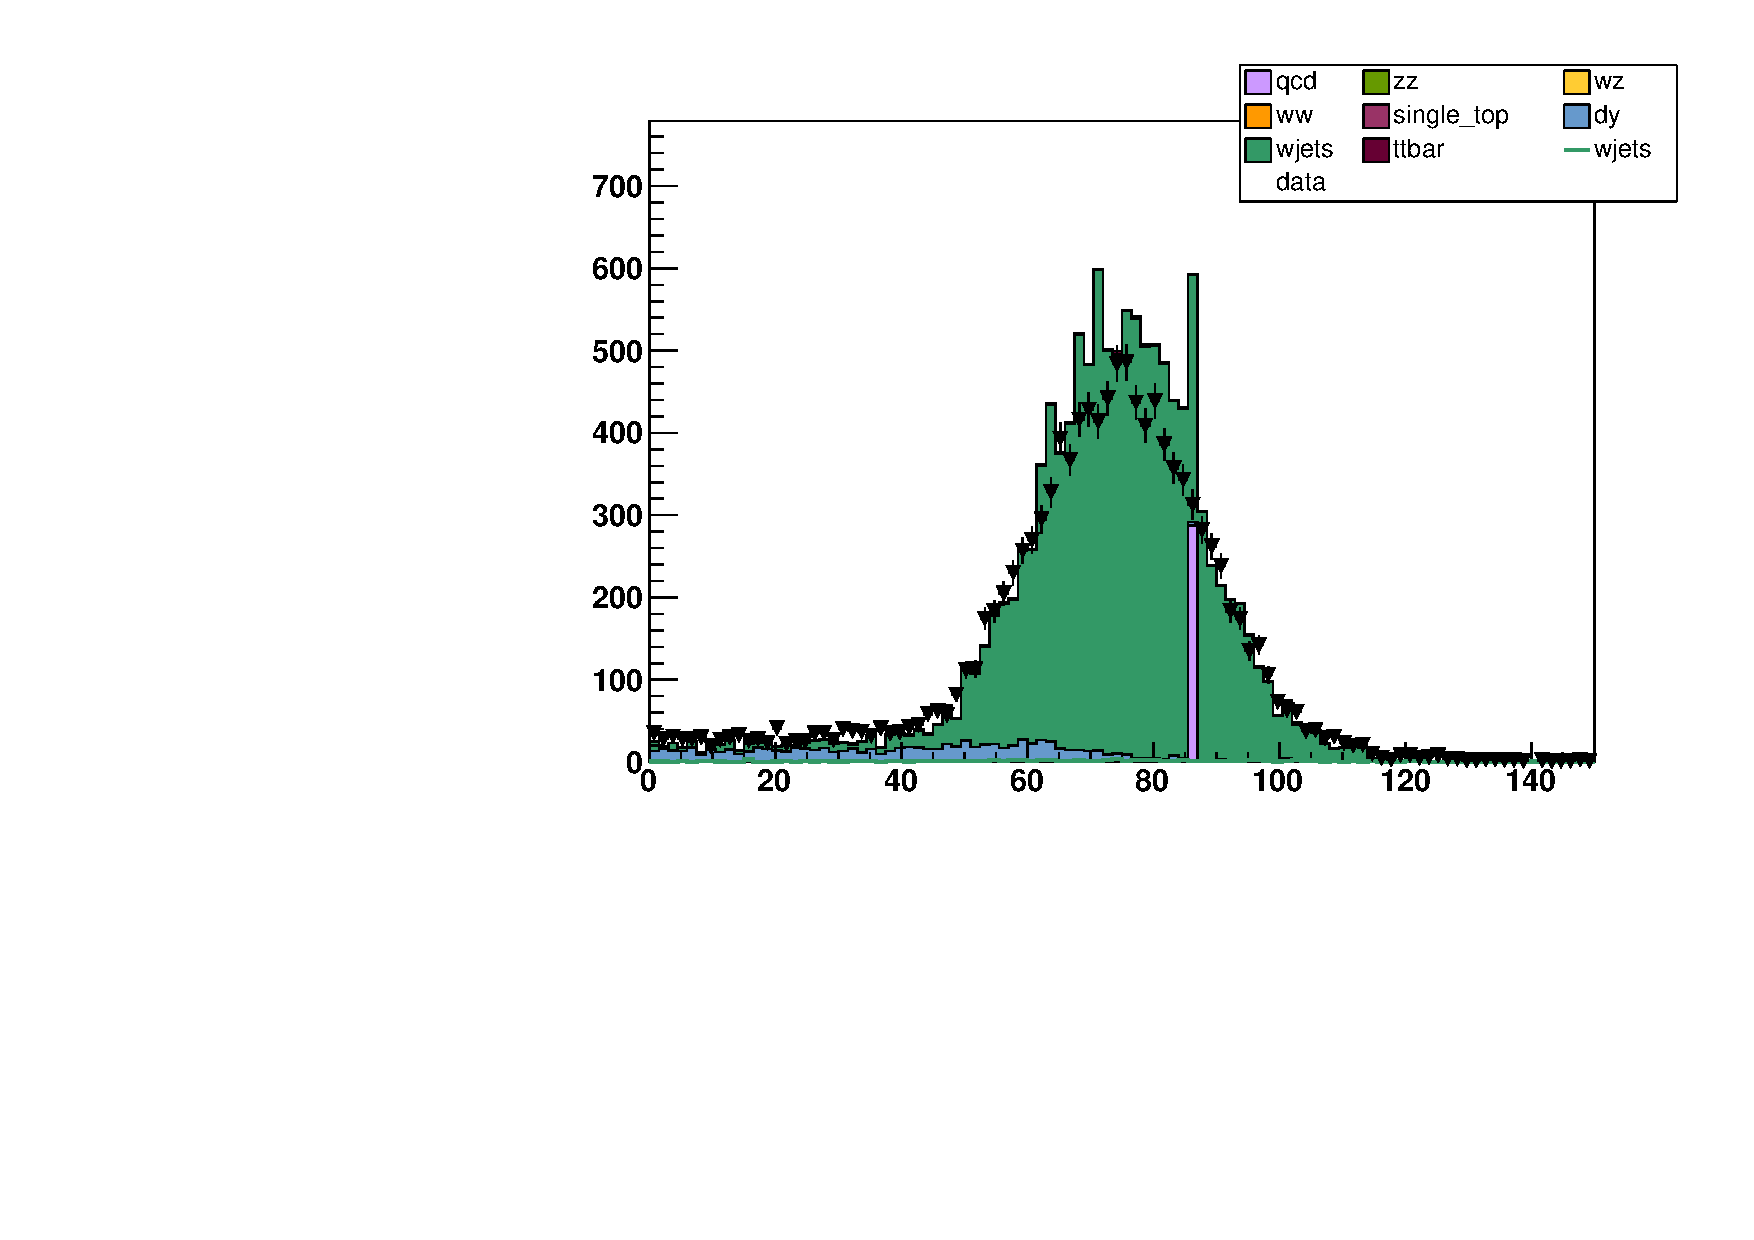
\includegraphics[width=\textwidth]{Plots/part2/W_mass_n.pdf}
            \caption{$W^-$-boson mass [GeV] distribution of the selected events.}    
            \label{fig:mean and std of net24}
        \end{subfigure}
        \vskip\baselineskip
        \begin{subfigure}[b]{0.475\textwidth}   
            \centering 
            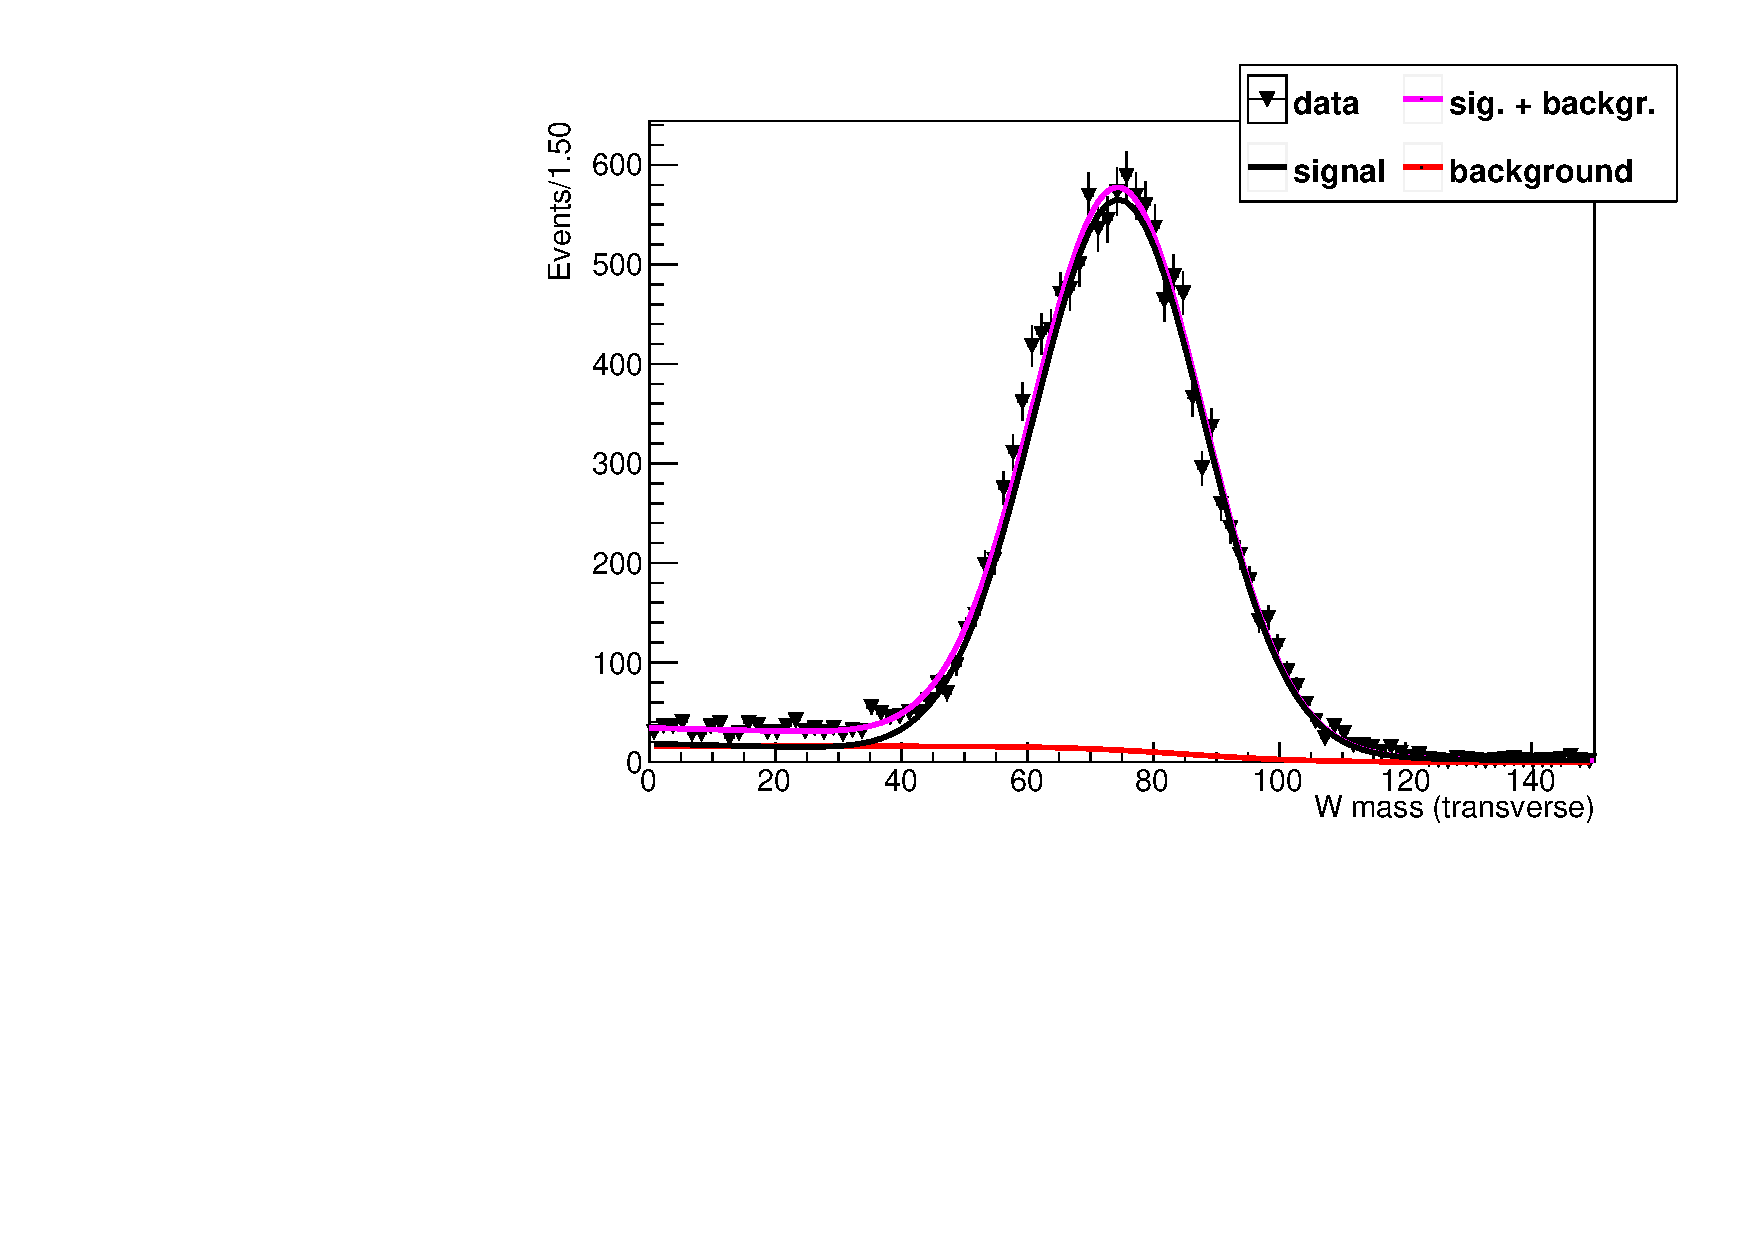
\includegraphics[width=\textwidth]{Plots/part2/sig_fit_bkg_positive_0.pdf}
            \caption{Total fit on the events containing a $\mu^+$, including the contributions of the MC estimated background and signal.}   
            \label{fig:mean and std of net34}
        \end{subfigure}
        \hfill
        \begin{subfigure}[b]{0.475\textwidth}   
            \centering 
            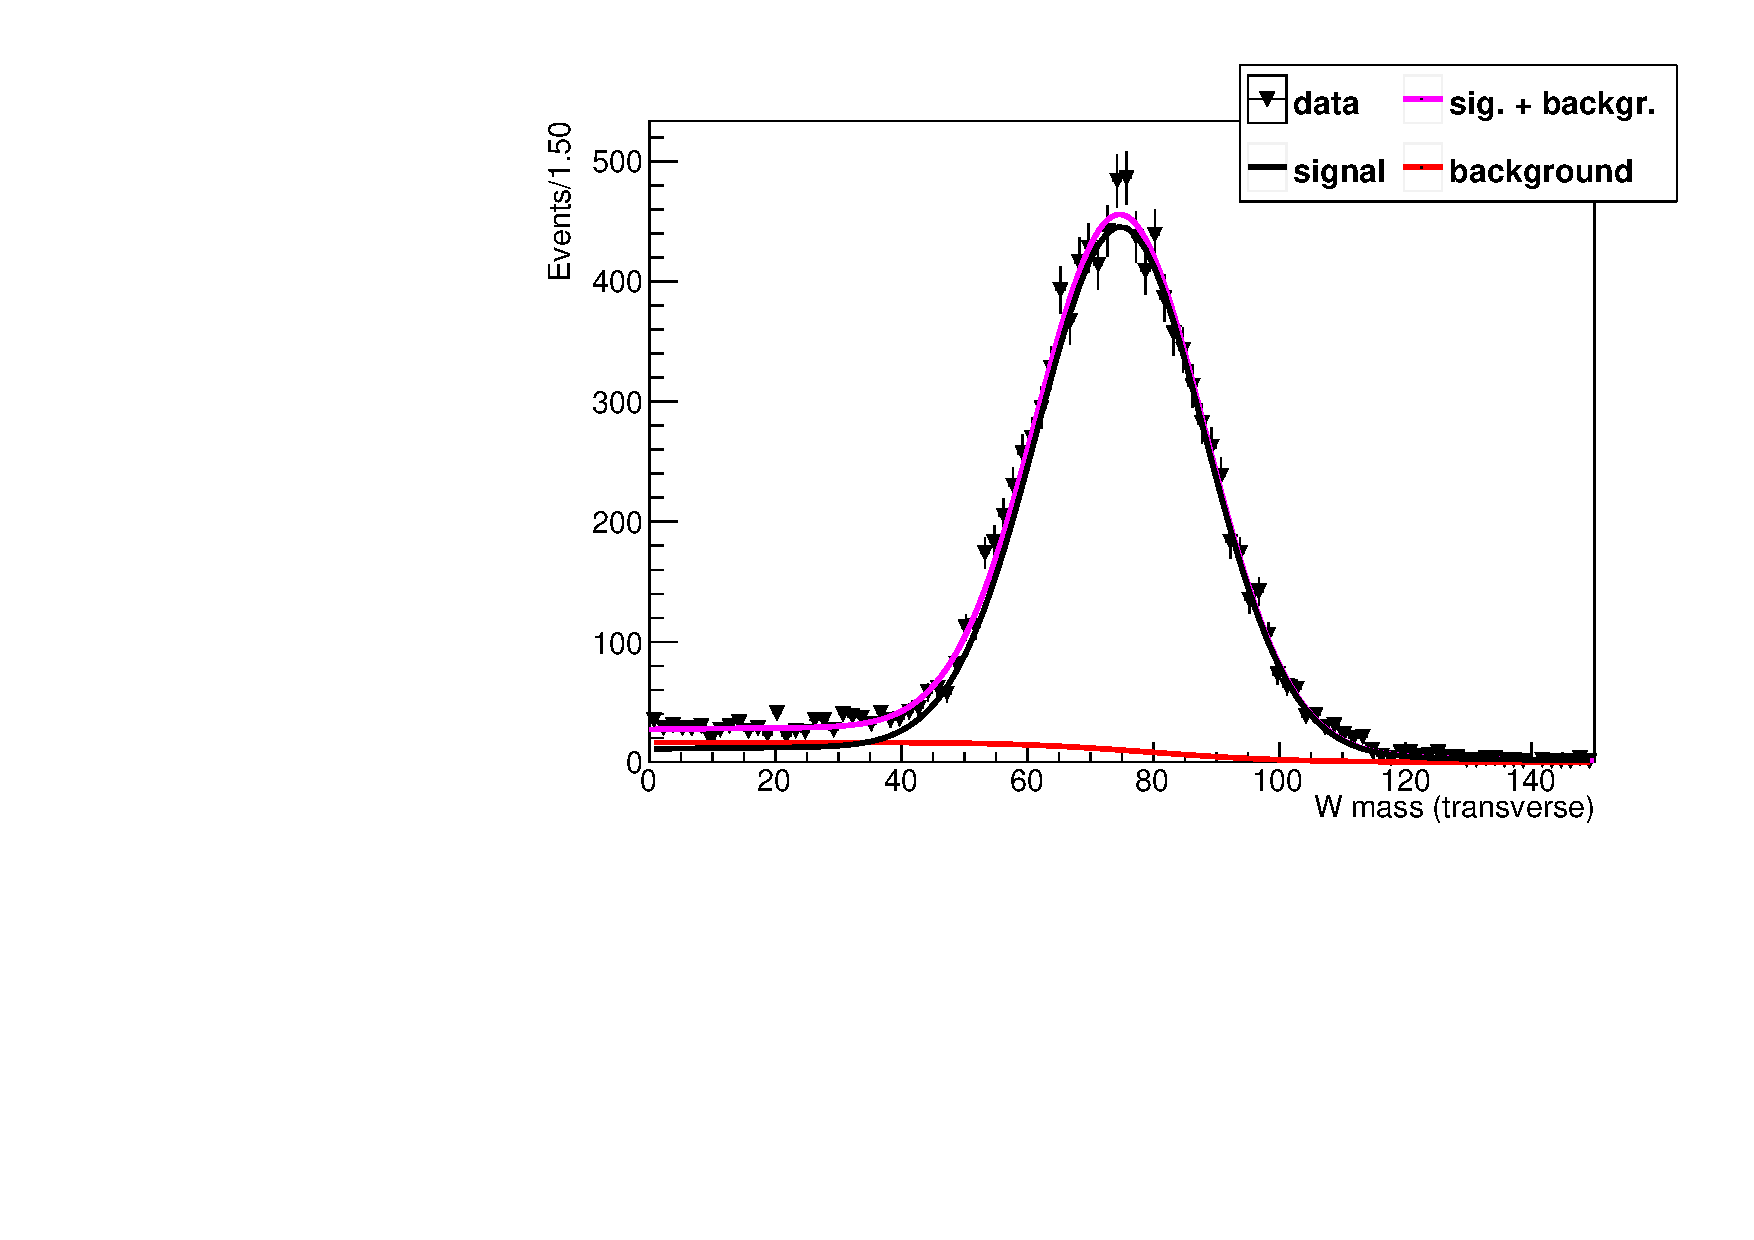
\includegraphics[width=\textwidth]{Plots/part2/sig_fit_bkg_negative_0.pdf}
            \caption{Total fit on the events containing a $\mu^-$, including the contributions of the MC estimated background and signal.}   
            \label{fig:mean and std of net44}
        \end{subfigure}
        \caption{Plot results of the W-boson charge asymmetry for a pseudorapidity $< 0.4$ The left row indicates events with a positive muon and the right row events with a negative muon. The upper figures show that the event selection was very accurate, as the main background comes from Drell-Yan processes. The single bar indicating a high QCD background is most likely an artifact, as the histograms are weighted.}
        \label{fig:W_asym}
\end{figure*}



\section{Results and Outlook}

The total cross-section for the event $t \bar t \rightarrow \mu \nu b \bar b q \bar q$ of 
$(155.6 \, \pm \, 21.0$ (stat.) $\pm \, 15.6$ (sys.)$)$ pb agrees with the literature value of $(173.6 \, \pm \, 11.7)$ pb \cite{workman_review_2022}. This measurement was not very accurate, but fairly precise. The cut selection can be improved, as relatively few events passed the selection criteria. I would have liked to select events with at least two b-jets, but then there would have been even less events left.
On the other hand, if the cuts are less strict, there would be more background events passing the selection. For more precise and accurate results, one should use a more systematic approach for selecting the cuts. \\
The W-boson charge asymmetry of $(11.3 \pm 0.9)$ \% for a $\eta < 0.4$ agrees well with the literature, as does the general trend of larger $\mathcal{A}$ with increasing $\eta$. The MC background does seem to have some signal at 60 GeV in it. Further investigation would be required to explain this behaviour. 








\section{Error propagation}

The uncertainties were consistently calculated using Gaussian error propagation. 
The uncertainty on the cross-section is given by:

\begin{multline}\label{eq:cross_sec_err}
    \sigma_{\sigma}^{1/2} = \left(\frac{\partial \sigma}{\partial N}\right)^2 \cdot \sigma_N^2 + \left(\frac{\partial \sigma}{\partial L}\right)^2 \cdot \sigma_L^2 \\
    + \left(\frac{\partial \sigma}{\partial \epsilon}\right)^2 \cdot \sigma_{\epsilon}^2 + \left(\frac{\partial \sigma}{\partial A}\right)^2 \cdot \sigma_A^2 \\
    = \left(\frac{1}{L \epsilon A}\right)^2 \cdot \sigma_N^2 + \left(\frac{N}{L^2 \epsilon A}\right)^2 \sigma_L^2 \\
    + \left(\frac{N}{L \epsilon^2 A}\right)^2 \cdot \sigma_{\epsilon}^2 + \left(\frac{N}{L \epsilon A^2}\right)^2 \cdot \sigma_A^2
\end{multline}


The error on the score is given by equation \ref{eq:score_err}:

\begin{multline}\label{eq:score_err}
    \sigma_{\varsigma}^{1/2} = \left(\frac{\partial \varsigma}{\partial S}\right)^2 \cdot \sigma_S^2 + \left(\frac{\partial \varsigma}{\partial B}\right)^2 \cdot \sigma_B^2 \\
    = \left(\frac{\sqrt{S + B} - \frac{S}{2\sqrt{S+B}}}{S + B }\right)^2 \cdot \sigma_S^2 + \left(\frac{S}{2 \left(S+B\right)^{3/2}}\right)^2 \cdot \sigma_B^2
\end{multline}

Where S indicates the number of events identified as signal, B is the number of events identified as background, and $\sigma_{S,B}$ is the uncertainty on the signal/background.

The uncertainty on the charge asymmetry is given by the following equation:

\begin{multline}\label{eq:charge_asym_err}
    \sigma_{\mathcal{A}} = \sqrt{
    \left(\frac{\partial \mathcal{A}}{\partial N_+}\right)^2 \cdot \sigma_{N_+}^2 + \left(\frac{\partial \mathcal{A}}{\partial N_-}\right)^2 \cdot \sigma_{N_-}^2
    } 
    = \\ 
    \sqrt{
    \left(\frac{2 N_-}{\left(N_+ + N_- \right)}\right)^2 \cdot \sigma_{N_+}^2 + \left(\frac{2 N_+}{\left(N_+ + N_- \right)}\right)^2 \cdot \sigma_{N_-}^2
    } 
\end{multline}

Here, $N_{+/-}$ is the number of events including a $\mu^{+/-}$, as indicated in section \ref{sec:introduction}, with uncertainty $\sigma_{N_{+/-}}$


\bibliographystyle{apsrev4-1}
\bibliography{EPP}

\end{document}

